\subsection{Exact-v16 candidate-region variable comparisons}
\label{app:v4p3-candidate-region-comparisons}

The exact-v16 mass--control surfaces permit one common regional comparison at
six catalogue anchors inside their support: 51, 65, 80, 90, 117, and
162~MeV.  The 21 and 39~MeV entries are omitted solely because these surfaces
begin at 40~MeV; the omission is a surface-support choice and not an ordering
of the catalogue features.  The displayed quantities are overlap-weighted
histogram approximations to normalized selected-row shapes and category
fractions.  They do not define a fitted signal yield, significance, or limit.

For anchor $m_0$ and the frozen resolution $\sigma_m(m_0)$, define the
half-open lower, central, and upper regions
\begin{equation}
\begin{aligned}
 \mathcal{L}(m_0) &=[m_0-4\sigma_m,\,m_0-2.5\sigma_m), \\
 \mathcal{C}(m_0) &=[m_0-2.5\sigma_m,\,m_0+2.5\sigma_m), \\
 \mathcal{U}(m_0) &=[m_0+2.5\sigma_m,\,m_0+4\sigma_m).
\end{aligned}
\label{eq:v4p3-candidate-region-windows}
\end{equation}
For native 0.125-MeV mass bin $i$ with edges $[a_i,b_i)$, its contribution
to region $R$ is weighted by
\begin{equation}
 w_{iR}=\frac{\left|[a_i,b_i)\cap R\right|}{b_i-a_i}.
 \label{eq:v4p3-region-overlap-weight}
\end{equation}
Thus a region total or control-bin count is a fractional edge-overlap sum,
$N_{Rj}=\sum_i w_{iR}N_{ij}$, rather than a native-bin-center selection.
Every regional distribution is normalized independently,
$p_{Rj}=N_{Rj}/\sum_kN_{Rk}$, so the comparison concerns shape rather than
the rapidly varying mass yield.  Because the two sidebands have equal width,
their symmetric first-order local reference is the composition chord
\begin{equation}
 p_{{\rm chord},j}=\frac{p_{\mathcal{L},j}+p_{\mathcal{U},j}}{2},\qquad
 \Delta_j=100\left(p_{\mathcal{C},j}-p_{{\rm chord},j}\right),\qquad
 \mathrm{TV}=\frac{1}{2}\sum_j
 \left|p_{\mathcal{C},j}-p_{{\rm chord},j}\right|.
 \label{eq:v4p3-region-comparison-statistics}
\end{equation}
Here $\Delta_j$ is a percentage-point shape residual and TV is a descriptive
distance.  Neither is a pull or calibrated test statistic.

For continuous controls, display groups are frozen from rows outside the
union of all six fractional central regions and then reused without retuning
at individual anchors.  This prevents any one catalogue window from setting
the display-bin edges.  The six surfaces reuse selected rows, so comparisons
across variables are correlated descriptions of the same production.

The 65 and 80~MeV central windows are disjoint: the first ends at
70.304~MeV and the second begins at 74.280~MeV.  Their adjacent sidebands
overlap from 70.849 to 73.487~MeV and therefore sample part of the same
neighboring deficit/background interval.  The 80 and 90~MeV central windows
overlap from 83.950 to 85.720~MeV, and their adjacent sidebands also cross
into the neighboring central interval.  The anchor panels are consequently
regional views, not a partition into disjoint selected-row samples.

For validation at 65 and 80~MeV, the baseline-closed momentum-sum,
electron-hit, topology, and trigger surfaces have overlap-weighted central
totals of 16,361,498 and 20,983,869 rows, compared with the parser-exact
totals of 16,361,818 and 20,984,092.  The corresponding overlap-weighted
combined-sideband totals are 9,193,205 and 12,256,152 rows, compared with
parser-exact values of 9,193,162 and 12,255,727.  These few-$10^{-5}$ relative
differences are the expected consequence of applying continuous window edges
to saved mass histograms.  The vertex-significance and minimum-$|y_0|$
surfaces retain their separately recorded control-axis flow qualifications;
their per-surface totals are given in the machine-readable ledger.

\subsubsection{Saved control-variable shapes}
\label{app:v4p3-candidate-region-continuous}

Figures~\ref{fig:v4p3-candidate-region-psum}--
\ref{fig:v4p3-candidate-region-electron-n3d-hits} apply the same region
geometry and grouping ledger to three continuous controls and the stored
discrete electron 3D-hit count.  Lower and upper sidebands remain separate,
while the chord supplies a symmetric local reference.

\begin{figure}[H]
\centering
\graphicorplaceholder{0.98\linewidth}{final_limit_projection_figs/v4p3_candidate_region_variable_comparisons_20260811/candidate_region_psum.pdf}
\caption{Overlap-weighted, normalized pair-momentum-sum distributions in the
central, lower-sideband, and upper-sideband regions at 51, 65, 80, 90, 117,
and 162~MeV, with the equal-sideband chord as the local shape reference.}
\label{fig:v4p3-candidate-region-psum}
\end{figure}

\begin{figure}[H]
\centering
\graphicorplaceholder{0.98\linewidth}{final_limit_projection_figs/v4p3_candidate_region_variable_comparisons_20260811/candidate_region_vtx_proj_sig.pdf}
\caption{Overlap-weighted, normalized vertex-projection-significance
distributions and chord references in the same six regions.  Vertex-
projection significance is not reconstructed vertex $z$.}
\label{fig:v4p3-candidate-region-vtx-proj-sig}
\end{figure}

\begin{figure}[H]
\centering
\graphicorplaceholder{0.98\linewidth}{final_limit_projection_figs/v4p3_candidate_region_variable_comparisons_20260811/candidate_region_min_y0.pdf}
\caption{Overlap-weighted, normalized minimum-track $|y_0|$-proxy
distributions and chord references in the same six regions.  Display groups
are frozen with the union of all six central regions masked.}
\label{fig:v4p3-candidate-region-min-y0}
\end{figure}

\begin{figure}[H]
\centering
\graphicorplaceholder{0.98\linewidth}{final_limit_projection_figs/v4p3_candidate_region_variable_comparisons_20260811/candidate_region_electron_n3d_hits.pdf}
\caption{Overlap-weighted, normalized stored electron-track 3D-hit-count
distributions and chord references in the same six regions.  This quantity is
distinct from the N2D-hit variable used in earlier selection studies.}
\label{fig:v4p3-candidate-region-electron-n3d-hits}
\end{figure}

\subsubsection{Exhaustive category comparisons}
\label{app:v4p3-candidate-region-categories}

The topology panels use the six exhaustive saved categories, including
\texttt{topology\_other}.  The stored-trigger panels use the three populated
flag categories; they summarize stored flag combinations rather than
independent trigger samples.  Exact partition closure is inherited from the
release-level checks in Table~\ref{tab:v4p3-v16-provenance}.

\begin{figure}[H]
\centering
\graphicorplaceholder{0.98\linewidth}{final_limit_projection_figs/v4p3_candidate_region_variable_comparisons_20260811/candidate_region_topology.pdf}
\caption{Overlap-weighted topology fractions and chord references in the
central and adjacent-sideband regions at all six supported anchors.  Each
regional category vector is normalized to unity.}
\label{fig:v4p3-candidate-region-topology}
\end{figure}

\begin{figure}[H]
\centering
\graphicorplaceholder{0.98\linewidth}{final_limit_projection_figs/v4p3_candidate_region_variable_comparisons_20260811/candidate_region_trigger.pdf}
\caption{Overlap-weighted stored-trigger-category fractions and chord
references in the same six regions.  Each regional category vector is
normalized to unity.}
\label{fig:v4p3-candidate-region-trigger}
\end{figure}

\begin{figure}[H]
\centering
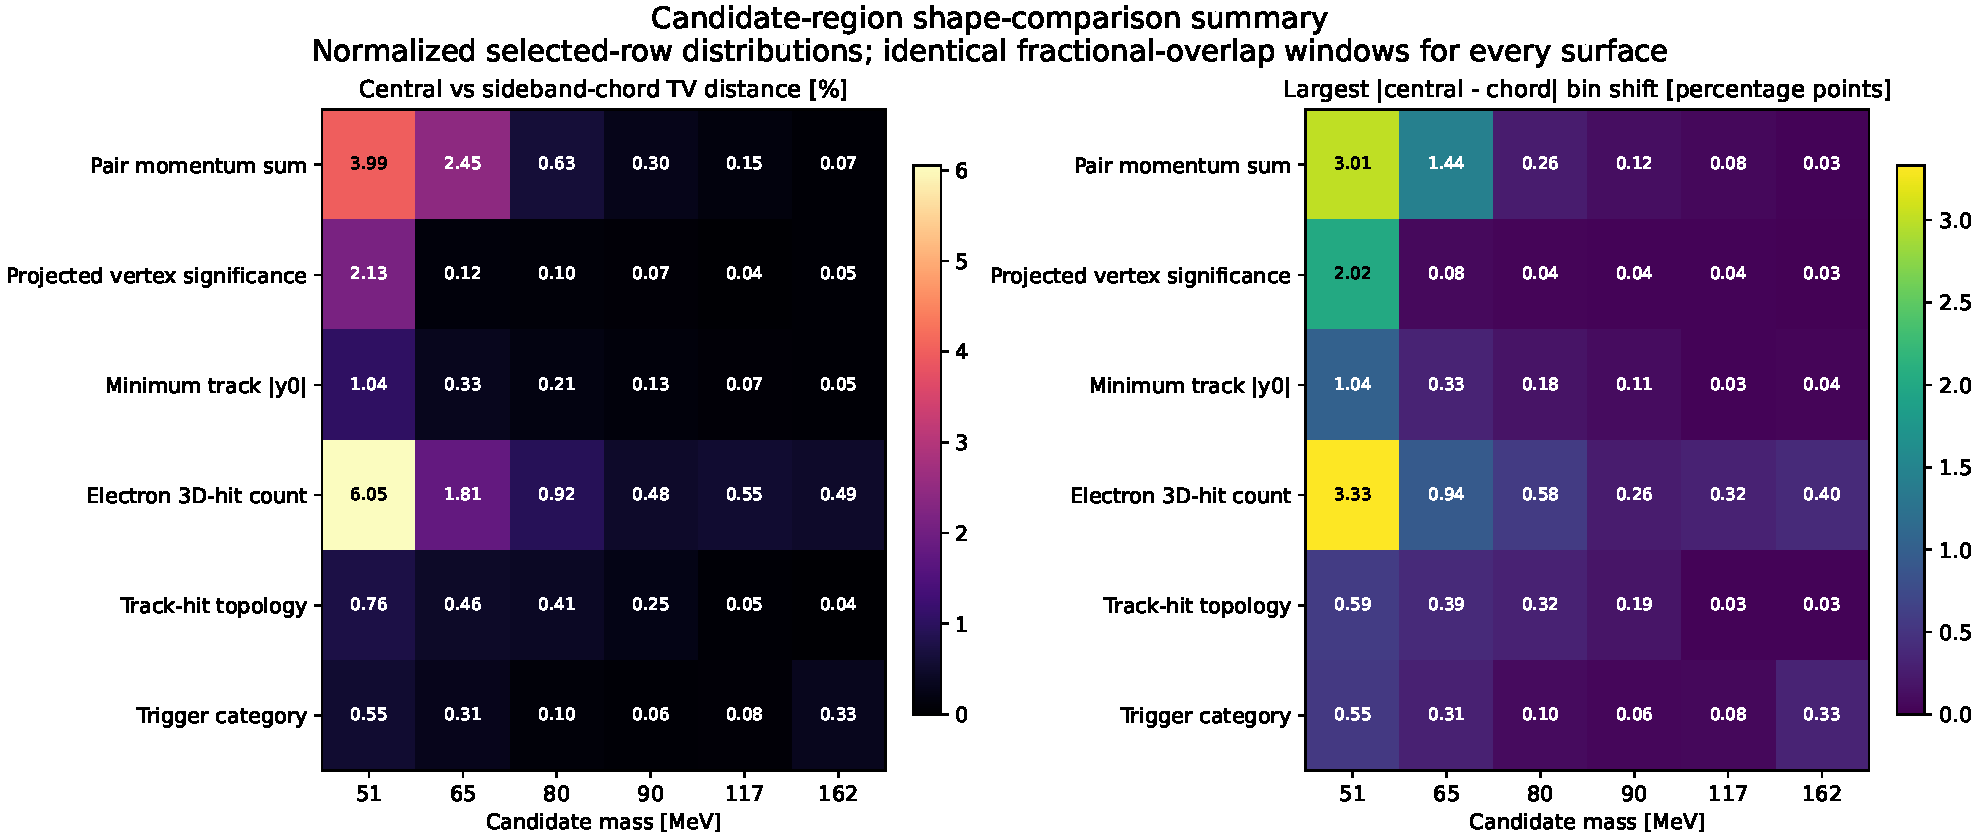
\includegraphics[width=0.98\linewidth]{final_limit_projection_figs/v4p3_candidate_region_variable_comparisons_20260811/candidate_region_tv_summary.pdf}
\caption{Total-variation distances between each overlap-weighted normalized
central-region distribution and the equal-sideband composition chord.  Values
are descriptive shape distances; they are not pulls, $p$-values, or
confidence intervals.}
\label{fig:v4p3-candidate-region-tv-summary}
\end{figure}

The summary in Figure~\ref{fig:v4p3-candidate-region-tv-summary} makes the
mass ordering quantitative.  At 51~MeV, the chord TV distances are 3.99\%
for momentum sum, 2.13\% for vertex-projection significance, 1.04\% for
minimum $|y_0|$, and 6.05\% for electron hit count; this is the strongest
left-to-right evolution and coincides with the lower-boundary/selection
turn-on region.  At 65~MeV the largest distances are 2.45\% in momentum sum
and 1.81\% in hit count, with 0.46\% in topology and 0.31\% in stored-trigger
composition.  The corresponding 80~MeV distances are smaller: 0.63\%,
0.92\%, 0.41\%, and 0.10\%, respectively.  The 90 and 117~MeV central shapes
closely interpolate their adjacent sidebands.  At 162~MeV the control and
topology distances remain small, with 0.49\% in hit count and 0.33\% in the
stored-trigger composition; this anchor is retained as a direct morphology
comparison beyond the current 40--160~MeV primary conditional-GPR domain.

The reciprocal 65/80 response reported by the frozen v4.2 inpainting/refit
is interpreted separately from these direct shape comparisons.  It is a
model-mediated response of the common nonlocal GP/background profile and can
be transmitted by the adjacent deficit/background structure.  The present
plots therefore retain 65 and 80~MeV as distinct local regions while avoiding
a physical-dependence interpretation.

The region comparisons keep both adjacent sidebands visible and use one
frozen grouping rule across anchors.  This supports like-for-like visual and
numerical comparisons while retaining ordinary mass evolution in the record.
Interpretation remains limited to the saved histogram axes and their
selected-row population; the plots do not supply an event-level signal
response or inferential calibration.
